% !TeX root = er.tex

\chapter{Traitement des Images}\label{ch.image}
\index{traitement des images}

Le capteur de distance de votre voiture autonome détecte un objet à $100$ mètres devant votre voiture. Suivez-vous la voiture qui vous précède à une distance sûre ou un piéton a-t-il sauté sur la route ? Les algorithmes robotiques présentés jusqu'à présent reposent sur la mesure de propriétés physiques telles que la distance, les angles et la réflectance. Les tâches plus complexes exigent qu'un robot obtienne des informations détaillées sur son environnement, en particulier lorsque le robot est destiné à fonctionner de manière autonome dans un environnement inconnu.

Pour nous, la façon la plus évidente d'appréhender notre environnement est d'utiliser la vision. Nous tenons la vision pour acquise et ne réalisons pas à quel point notre système visuel - nos yeux et notre cerveau - est complexe. En fait, environ $30\%$ du cerveau est utilisé pour la vision. Nous pouvons distinguer instantanément une voiture en mouvement d'un piéton qui traverse la route et réagir rapidement.

Depuis près de deux cents ans, il est possible d'enregistrer automatiquement des images à l'aide d'un appareil photo, mais l'interprétation des images reste une tâche qui incombe à l'homme. Avec l'avènement des ordinateurs, il est devenu possible de traiter et d'interpréter automatiquement les images. Les images numériques nous sont familières : les cartes météorologiques transmises par les satellites, les images médicales (radiographies, tomodensitogrammes, IRM, échographies) et les photos que nous prenons avec nos smartphones. Le traitement des images numériques est l'un des domaines les plus étudiés de l'informatique et de l'ingénierie, mais les capacités des systèmes de traitement d’images restent actuellement inférieures à celles du système visuel humain.

Dans ce chapitre, nous présentons un aperçu des algorithmes de traitement des images numériques et décrivons comment ils sont utilisés dans les systèmes robotiques. Les sections~\ref{s.obtaining-images}--\ref{s.image-overview} donnent un aperçu des systèmes d'imagerie et du traitement numérique des images. Les sections~\ref{s.enhance}--\ref{s.blob} décrivent les algorithmes de traitement des images : amélioration par filtres numériques et manipulation de l'histogramme, segmentation (détection des bords), et reconnaissance des caractéristiques (détection des coins et des blobs, identification des caractéristiques multiples).

Pour des raisons de coût et de puissance de calcul, peu de robots éducatifs utilisent des caméras. Pour étudier les algorithmes de traitement d'images, vous pouvez donc les implémenter sur un ordinateur personnel en utilisant des images capturées avec un appareil photo numérique. Néanmoins, nous proposons quelques activités qui mettent en œuvre les algorithmes de traitement d’images avec un robot éducatif. Le robot se déplace sur une image unidimensionnelle et des échantillons sont lus par un capteur au sol. Il en résulte un tableau unidimensionnel de pixels qui peut être traité à l'aide de versions simplifiées des algorithmes que nous présentons.

\section{Obtention d'images}\label{s.obtaining-images}

Dans cette section, nous donnons un aperçu des considérations relatives à la conception des systèmes d'imagerie.

\subsection*{Optique}
\index{traitement d'images!optique}
Le système optique d'un appareil photo se compose d'un objectif qui concentre la lumière sur un capteur. Plus l'objectif est large, plus il peut capter de lumière, ce qui est important pour les systèmes qui doivent travailler dans des environnements sombres. Plus la longueur focale (qui est liée à la distance entre l'objectif et le capteur) est grande, plus le grossissement est important. C'est pourquoi les photographes professionnels portent des appareils photo lourds, dotés de longs objectifs. Les fabricants de smartphones sont confrontés à un dilemme : nous voulons que nos téléphones soient fins et élégants, mais cela limite la longueur focale de l'appareil photo. Pour la plupart des applications en robotique, la taille et le poids nécessaires pour obtenir une longue distance focale sont tels qu’ils ne contrebalancent pas le gain en grossissement.

\subsection*{Résolution}
\index{traitement des images!résolution}

Il fut un temps où les images étaient capturées sur pellicule par une réaction chimique provoquée par la lumière frappant une feuille de plastique recouverte d'une émulsion de minuscules particules d'argent. En principe, chaque particule pouvait réagir indépendamment, de sorte que la résolution était extrêmement élevée. Dans les images numériques, la lumière est captée par des dispositifs semi-conducteurs tels que les dispositifs à couplage de charge (CCD). Un appareil photo numérique contient une puce avec un nombre fixe d'éléments dans un tableau rectangulaire. Chaque élément mesure l'intensité lumineuse de manière indépendante et ces mesures sont appelées \emph{pixels}. Pour une surface donnée, plus il y a de pixels capturés par une puce, plus la résolution est élevée. Actuellement, même les appareils photo bon marché des smartphones peuvent capturer des millions de pixels dans une seule image.

Le problème des images à haute résolution est la grande quantité de mémoire nécessaire pour les stocker. Prenons l'exemple d'un écran d'ordinateur à haute résolution avec $1\:920 \times 1\:080$ pixels et supposons que chaque pixel utilise $8$ bits pour stocker l'intensité dans la plage $0$--$255$. Une seule image nécessite environ $2$ mégaoctets (Mo) de mémoire. Avec cette résolution, un ordinateur embarqué ne peut analyser qu’une seule image de ce type, mais un robot mobile peut avoir besoin de stocker plusieurs images par seconde.

Un point encore plus important que la quantité de mémoire requise est la puissance de calcul nécessaire pour analyser les images. Les algorithmes de traitement d'images exigent que l'ordinateur effectue un calcul sur chaque pixel. Ce n'est pas un problème pour un astronome qui analyse des images envoyées vers la terre par un télescope spatial, mais c'est un problème pour une voiture autonome qui doit prendre des décisions en une fraction de seconde.

\subsection*{Couleur}
\index{traitement des images!couleur}

Notre système visuel est capable de distinguer une plage de longueurs d'onde appelée \emph{lumière visible}. Les différentes longueurs d'onde sont perçues comme des couleurs différentes. La lumière de grande longueur d'onde est appelée \emph{rouge}, tandis que la lumière de petite longueur d'onde est appelée \emph{violet}. L'œil humain peut distinguer des millions de couleurs différentes, même si nous n'en nommons que quelques-unes : rouge, orange, jaune, vert, cyan, bleu, violet, etc. La couleur est l'un des principaux outils que nous utilisons pour identifier les objets.

Les capteurs sont capables de mesurer la lumière à des longueurs d'onde situées en dehors de la plage que nous appelons lumière visible : \emph{infrarouge} pour les grandes longueurs d'onde et \emph{ultraviolet} pour les courtes longueurs d'onde. Les images infrarouges sont importantes en robotique, car les objets chauds tels que les personnes et les voitures peuvent être détectés sous forme de lumière infrarouge brillante.

Le problème de la couleur est qu'elle triple les exigences en matière de stockage et de traitement des images. Toutes les couleurs peuvent être formées en prenant des quantités variables des trois \emph{couleurs primaires} : rouge, vert et bleu (RVB). Par conséquent, une image couleur nécessite trois octets pour chaque pixel. Le stockage d'une seule image couleur d'une résolution de $1\:920 \times 1\:080$ nécessite plus de $6$ Mo de mémoire et le temps de traitement de l’image est au moins triplé.

\section{Une aperçu du traitement numérique des images}\label{s.image-overview}

Le système optique d'un robot capture des images sous forme de tableaux rectangulaires de pixels, mais les tâches d'un robot sont exprimées en termes d'objets de l'environnement : entrer dans une pièce par une porte, prendre un article sur une étagère, s'arrêter si un piéton traverse devant la voiture. Comment passer des pixels aux objets ?

La première étape est l'\emph{amélioration de l'image}\index{traitement de l'image!amélioration}. Les images contiennent du bruit qui provient de l'optique et de l'électronique. De plus, l'éclairage de l'environnement peut rendre une image trop sombre ou délavée ; l'image peut être tournée accidentellement ; l'image peut être floue. Tous ces problèmes sont indépendants de son contenu. Il importe peu qu'une image floue représente un chat ou un enfant. Les algorithmes d'amélioration d'image agissent généralement en modifiant les valeurs attribuées à chaque pixel, sans tenir compte de leur signification. \footnote{Il existe une autre approche, appelée algorithmes de traitement \emph{fréquence}, mais elle fait appel à des techniques mathématiques qui dépassent le cadre de cet ouvrage.}

L'amélioration des images est difficile car il n'existe pas de définition formelle de ce que signifie améliorer une image. Une tache floue peut être de la saleté sur l'objectif d'un appareil photo ou une galaxie inconnue. La section~\ref{s.enhance} présente deux approches de l'amélioration d'image : le filtrage qui supprime le bruit en remplaçant un pixel par une moyenne de ses pixels voisins et la manipulation de l'histogramme qui modifie la luminosité et le contraste d'une image.

Les objets se distinguent par des lignes, des courbes et des zones. Une porte est caractérisée par trois bords droits d’un rectangle auquel il manque un petit côté. Un feu de circulation est constitué de trois disques lumineux les uns au-dessus des autres. Avant de pouvoir identifier une porte ou un feu de signalisation, les algorithmes de traitement d'image permettent de déterminer quels pixels représentent des lignes, des bords, etc. Ce processus est appelé \emph{segmentation}\index{traitement d'image!segmentation} ou \emph{extraction de caractéristiques} car les algorithmes servent à détecter et classer les pixels en fonction de critères donnés. L'identification des pixels qui composent les bords d'une image est ainsi rendue possible.

La segmentation serait facile si les bords, les lignes et les courbes étaient uniformes, mais ce n'est pas le cas dans les images réelles. Un bord peut être incliné à un angle arbitraire et certains de ses pixels peuvent être masqués par des ombres ou même disparaître. Les \emph{captchas} sont un exemple bien connu où les lettres sont intentionnellement déformées pour rendre la reconnaissance automatique très difficile alors que les humains peuvent facilement identifier des lettres déformées. Les algorithmes d'amélioration peuvent faciliter la segmentation, par exemple en complétant les pixels manquants, mais ils peuvent également introduire des segments artificiels. La section~\ref{s.edge-detection} présente une technique de segmentation : un filtre qui détecte les bords d'une image.

La dernière phase du traitement d'images consiste à reconnaître les objets. Dans la section \ref{s.corners}, nous présentons deux algorithmes de détection des coins : en localisant l'intersection de deux bords et en comptant les pixels voisins ayant des intensités similaires. La section~\ref{s.blob} décrit comment reconnaître les \emph{blobs}, qui sont des zones dont les pixels ont des intensités similaires mais dont la frontière n’a pas de caractéristiques régulières telles que des lignes ou des courbes. Enfin, l'activité \ref{act.recognize} présente la reconnaissance d'un objet défini par plus d'une caractéristique, comme une porte définie par deux bords situés à une distance arbitraire l'un de l'autre.

\section{Amélioration d'image}\label{s.enhance}
\index{traitement de l'image!amélioration}

La figure~\ref{fig.no-noise} montre l'image d'un rectangle dont l'intensité est uniforme horizontalement et dégradée de sombre à clair de haut en bas. La représentation de l'image sous la forme d'un tableau rectangulaire de pixels de $6 fois 10$ est illustrée dans la figure~\ref{fig.pixel-no-noise}, où chaque pixel est représenté par un niveau d'intensité lumineuse dans la plage $0$--$100$. Regardez maintenant la Fig.~\ref{fig.noise} : l'image n'est plus \emph{lisse} dans le sens où il y a trois points dont les intensités ne sont pas similaires à celles de leurs voisins respectifs. Comparez le tableau de pixels de la Fig.\ref{fig.pixel-noise} avec celui de la Fig.\ref{fig.pixel-no-noise} : les intensités des pixels aux positions $(2;3)$, $(3;6)$, $(4;4)$ sont différentes. Il s'agit probablement d'un bruit et non d'une réelle caractéristique de l'objet photographié. 

\begin{figure}
\begin{minipage}{.45\textwidth}

\begin{tikzpicture}
\shade[bottom color=black!40,top color=black!80] (0,0) rectangle +(4,1);
\end{tikzpicture}
\caption{Image sans bruit}\label{fig.no-noise}
\end{minipage}
\hspace{\fill}
\begin{minipage}{.45\textwidth}

\begin{tikzpicture}
\shade[bottom color=black!40,top color=black!80] (0,0) rectangle +(4,1);
\draw[fill,color=black!70] ( 8mm,5mm) rectangle +(1mm,1mm);
\draw[fill,color=black!80] (30mm,3mm) rectangle +(1mm,1mm);
\draw[fill,color=black!20] (15mm,2mm) rectangle +(1mm,1mm);
\end{tikzpicture}
\caption{Image avec bruit}\label{fig.noise}
\end{minipage}
\end{figure}

\begin{figure}
\begin{minipage}{.5\textwidth}
\begin{tabular}{r@{\hspace{4pt}}r@{\hspace{4pt}}r@{\hspace{4pt}}r@{\hspace{4pt}}r@{\hspace{4pt}}r@{\hspace{4pt}}r@{\hspace{4pt}}r@{\hspace{4pt}}r@{\hspace{4pt}}r@{\hspace{4pt}}r}
& $\scriptstyle 0$ & $\scriptstyle 1$ & $\scriptstyle 2$ & $\scriptstyle 3$ & $\scriptstyle 4$ & $\scriptstyle 5$ & $\scriptstyle 6$ & $\scriptstyle 7$ & $\scriptstyle 8$ & $\scriptstyle 9$ \\
$\scriptstyle 0$ & $10$ & $10$ & $10$ & $10$ & $10$ & $10$ & $10$ & $10$ & $10$ & $10$\\
$\scriptstyle 1$ & $20$ & $20$ & $20$ & $20$ & $20$ & $20$ & $20$ & $20$ & $20$ & $20$\\
$\scriptstyle 2$ & $30$ & $30$ & $30$ & $30$ & $30$ & $30$ & $30$ & $30$ & $30$ & $30$\\
$\scriptstyle 3$ & $40$ & $40$ & $40$ & $40$ & $40$ & $40$ & $40$ & $40$ & $40$ & $40$\\                   
$\scriptstyle 4$ & $50$ & $50$ & $50$ & $50$ & $50$ & $50$ & $50$ & $50$ & $50$ & $50$\\
$\scriptstyle 5$ & $60$ & $60$ & $60$ & $60$ & $60$ & $60$ & $60$ & $60$ & $60$ & $60$\\
\end{tabular}
\caption{Tableau de pixels sans bruit}\label{fig.pixel-no-noise}
\end{minipage}
\hspace{\fill}
\begin{minipage}{.5\textwidth}
\begin{tabular}{r@{\hspace{4pt}}r@{\hspace{4pt}}r@{\hspace{4pt}}r@{\hspace{4pt}}r@{\hspace{4pt}}r@{\hspace{4pt}}r@{\hspace{4pt}}r@{\hspace{4pt}}r@{\hspace{4pt}}r@{\hspace{4pt}}r}
& $\scriptstyle 0$ & $\scriptstyle 1$ & $\scriptstyle 2$ & $\scriptstyle 3$ & $\scriptstyle 4$ & $\scriptstyle 5$ & $\scriptstyle 6$ & $\scriptstyle 7$ & $\scriptstyle 8$ & $\scriptstyle 9$ \\
$\scriptstyle 0$ & $10$ & $10$ & $10$ & $10$ & $10$ & $10$ & $10$ & $10$ & $10$ & $10$\\
$\scriptstyle 1$ & $20$ & $20$ & $20$ & $20$ & $20$ & $20$ & $20$ & $20$ & $20$ & $20$\\
$\scriptstyle 2$ & $30$ & $30$ & $30$ & \boldmath $20$ & $30$ & $30$ & $30$ & $30$ & $30$ & $30$\\
$\scriptstyle 3$ & $40$ & $40$ & $40$ & $40$ & $40$ & $40$ & \boldmath $10$ & $40$ & $40$ & $40$\\
$\scriptstyle 4$ & $50$ & $50$ & $50$ & $50$ & \boldmath $90$ & $50$ & $50$ & $50$ & $50$ & $50$\\
$\scriptstyle 5$ & $60$ & $60$ & $60$ & $60$ & $60$ & $60$ & $60$ & $60$ & $60$ & $60$\\
\end{tabular}
\caption{Tableau de pixels avec bruit}\label{fig.pixel-noise}
\end{minipage}
\end{figure}

L'origine du bruit n'a pas vraiment d'importance : l'objet lui-même, la poussière sur l'objectif de l'appareil photo, la non-uniformité du capteur ou le bruit dans l'électronique. Il est impossible de se débarrasser complètement du bruit, car nous ne pouvons jamais être sûrs qu'un pixel est un bruit ou une caractéristique réelle de l'objet, mais nous voulons améliorer l'image de manière à ce que le bruit ne soit plus remarquable.

\subsection{Filtres spatiaux}
\index{traitement d'images!filtre spatial}

Considérons la ligne $4$ du tableau de pixels de la Fig.~\ref{fig.pixel-noise} :
\[
50,\, 50,\, 50,\,50,\, 90,\, 50,\, 50,\, 50,\, 50,\, 50\,.
\]
\ref{fig.before-average} est un graphique de l'intensité lumineuse $f$ pour les pixels de cette ligne. Il est clair que l'un des pixels a une valeur aberrante parce que cette valeur diffère fortement de celle de ses voisins. Un programme peut faire en sorte que chaque pixel ressemble davantage a ses voisins et remplaçant l’intensité d’un pixel par la moyenne de son intensité et des intensités de ses voisins. Pour la plupart des pixels de la ligne, cela ne change pas leurs valeurs : $(50+50+50)/3=50$, mais le pixel de bruit et ses deux voisins reçoivent de nouvelles valeurs : $(50+90+50)/3\approx 60$ (Fig.~\ref{fig.after-average}). Le calcul de la moyenne donne à deux pixels des valeurs "erronées", mais dans l'ensemble, l'image sera visuellement améliorée car l'intensité du bruit sera réduite.

\begin{figure}
\begin{minipage}{.47\textwidth}
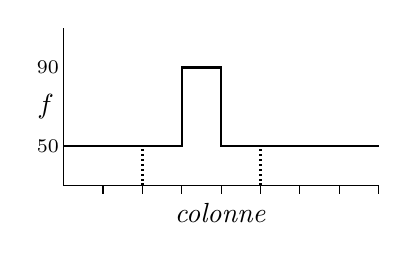
\begin{tikzpicture}[scale=1]
\draw (0,2) -- node[left] {$f$} (0,0) -- node[below,yshift=-1mm] {\textit{colonne}} (4,0);
\draw[thick] (0,.5) -- (1.5,.5) -- (1.5,1.5) -- (2,1.5) -- (2,.5) -- (4,.5);
\node at (-2mm,.5) {$\scriptstyle 50$};
\node at (-2mm,1.5) {$\scriptstyle 90$};
\foreach \x in {.5,1,1.5,2,2.5,3,3.5,4}
  \draw[thin] (\x,-1mm) -- (\x,0);
\draw[densely dotted,thick] (1,0) -- (1,.5);
\draw[densely dotted,thick] (2.5,0) -- (2.5,.5);
\end{tikzpicture}
\caption{Intensité avant le calcul de la moyenne}\label{fig.before-average}
\end{minipage}
\hspace{\fill}
\begin{minipage}{.47\textwidth}
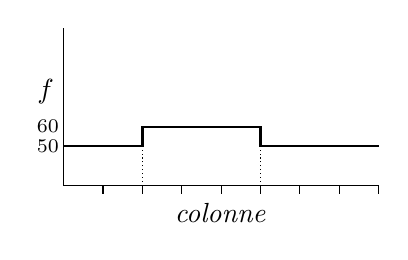
\begin{tikzpicture}[scale=1]
\draw (0,2) -- node[left,yshift=2mm] {$f$} (0,0) -- node[below,yshift=-1mm] {\textit{colonne}} (4,0);
\draw[thick] (0,.5) -- (1,.5) -- (1,.75) -- (2.5,.75) -- (2.5,.5) -- (4,.5);
\node at (-2mm,.5) {$\scriptstyle 50$};
\node at (-2mm,.75) {$\scriptstyle 60$};
\foreach \x in {.5,1,1.5,2,2.5,3,3.5,4}
  \draw[thin] (\x,-1mm) -- (\x,0);
\draw[densely dotted] (1,0) -- (1,.5);
\draw[densely dotted] (2.5,0) -- (2.5,.5);
\end{tikzpicture}
\caption{Intensité après le calcul de la moyenne}\label{fig.after-average}
\end{minipage}
\end{figure}

Prendre la moyenne d'une série de pixels est la version discrète de l'intégration d'une fonction d'intensité continue. L'intégration permet de lisser les variations locales de la fonction. Dans les figures \ref{fig.before-average} et \ref{fig.after-average}, on peut voir que les aires délimités par les droites en pointillés et sous la courbe d’intensité sont presque identiques pour la série des 3 pixels considérées.

Ce lissage est réalisée en appliquant un \emph{filtre spatial} à chaque pixel de l'image.\footnote{Le terme mathématique pour appliquer une fonction $g$ à chaque point d'une fonction $f$ est appelé \emph{convolution} (discrète). Pour les fonctions continues, l'intégration est utilisée à la place de l'addition de la moyenne.} Pour le tableau bidimensionnel de pixels, le filtre est représenté par un tableau de $3\times 3$, où chaque élément du tableau spécifie le facteur par lequel le pixel et ses voisins sont multipliés. Chaque pixel a quatre ou huit voisins, selon que l'on inclut ou non les voisins diagonaux. Ici, nous incluons les pixels diagonaux dans les filtres.

Le \emph{filtre de boîte}\index{traitement d'image!filtre de boîte} est :
\[
\left[
\begin{array}{ccc}
1 & 1 & 1\\
1 & 1 & 1\\
1 & 1 & 1
\end{array}
\right]\,.
\]
Ce filtre permet de multiplier chaque intensité par un coefficient donné (ici $1$) et de sommer ces $9$ produits. On divise par $9$ le résultat pour le ramener à une valeur d’intensité. 

L'application du filtre à chaque pixel $(r,c)$ peut s'écrire explicitement comme suit :
\[
\begin{array}{llll}
g(r,c) = &(\\
&f(r-1,c-1) & \;+\; f(r-1,c) & \;+\; f(r-1,c+1) \;+\\
&f(r,c-1) & \;+\; f(r,c) & \;+\; f(r,c+1) \;\;\;\;\;\;\;+\\
&f(r+1,c-1) & \;+\; f(r+1,c) & \;+\; f(r+1,c+1)\\
& ) \; / \; 9\,.
\end{array}
\]
La Fig.~\ref{fig.box-filter} montre le résultat de l'application du filtre en boîte à l'image bruitée de la Fig.~\ref{fig.pixel-noise}.\footnote{Le filtre n'est pas appliqué aux pixels des bords de l'image pour éviter de dépasser les limites du tableau. Une alternative est de compléter l’image par des lignes et des colonnes supplémentaires.} Les valeurs d'intensité ne sont plus uniformes, mais elles restent assez proches des valeurs d'origine, à part là où il y avait des pixels de bruit. La deuxième ligne en partant du bas montre que la valeur $90$ qui représentait un bruit n’apparaît plus ; au lieu de cela, toutes les valeurs de la ligne sont proches les unes des autres dans l'intervalle $[46 ; 54]$.

\begin{figure}
\begin{minipage}{.5\textwidth}
\begin{tabular}{r@{\hspace{4pt}}r@{\hspace{4pt}}r@{\hspace{4pt}}r@{\hspace{4pt}}r@{\hspace{4pt}}r@{\hspace{4pt}}r@{\hspace{4pt}}r@{\hspace{4pt}}r@{\hspace{4pt}}r@{\hspace{4pt}}r}
& $\scriptstyle 0$ & $\scriptstyle 1$ & $\scriptstyle 2$ & $\scriptstyle 3$ & $\scriptstyle 4$ & $\scriptstyle 5$ & $\scriptstyle 6$ & $\scriptstyle 7$ & $\scriptstyle 8$ & $\scriptstyle 9$ \\
$\scriptstyle 0$ & 10 & 10 & 10 & 10 & 10 & 10 & 10 & 10 & 10 & 10\\
$\scriptstyle 1$ & 20 & 20 & 18 & 18 & 18 & 20 & 20 & 20 & 20 & 20\\
$\scriptstyle 2$ & 30 & 30 & 28 & 28 & 28 & 26 & 26 & 26 & 30 & 30\\
$\scriptstyle 3$ & 40 & 40 & 38 & 43 & 43 & 41 & 36 & 36 & 40 & 40\\
$\scriptstyle 4$ & 50 & 50 & 50 & 54 & 54 & 51 & 46 & 46 & 50 & 50\\
$\scriptstyle 5$ & 60 & 60 & 60 & 60 & 60 & 60 & 60 & 60 & 60 & 60\\
\end{tabular}
\caption{Lissage avec le filtre en boîte}\label{fig.box-filter}
\end{minipage}
\hspace{\fill}
\begin{minipage}{.5\textwidth}
\begin{tabular}{r@{\hspace{4pt}}r@{\hspace{4pt}}r@{\hspace{4pt}}r@{\hspace{4pt}}r@{\hspace{4pt}}r@{\hspace{4pt}}r@{\hspace{4pt}}r@{\hspace{4pt}}r@{\hspace{4pt}}r@{\hspace{4pt}}r}
& $\scriptstyle 0$ & $\scriptstyle 1$ & $\scriptstyle 2$ & $\scriptstyle 3$ & $\scriptstyle 4$ & $\scriptstyle 5$ & $\scriptstyle 6$ & $\scriptstyle 7$ & $\scriptstyle 8$ & $\scriptstyle 9$ \\
$\scriptstyle 0$ & 10 & 10 & 10 & 10 & 10 & 10 & 10 & 10 & 10 & 10\\
$\scriptstyle 1$ & 20 & 20 & 19 & 19 & 19 & 20 & 20 & 20 & 20 & 20\\
$\scriptstyle 2$ & 30 & 30 & 29 & 25 & 29 & 28 & 28 & 28 & 30 & 30\\
$\scriptstyle 3$ & 40 & 40 & 39 & 41 & 41 & 40 & 25 & 38 & 40 & 40\\
$\scriptstyle 4$ & 50 & 50 & 50 & 52 & 70 & 50 & 48 & 48 & 50 & 50\\
$\scriptstyle 5$ & 60 & 60 & 60 & 60 & 60 & 60 & 60 & 60 & 60 & 60\\
\end{tabular}
\caption{Lissage avec un filtre pondéré}\label{fig.weighted-filter}
\end{minipage}
\end{figure}

Le filtre en boîte donne la même importance au pixel qu'à tous ses voisins, mais un \emph{filtre pondéré}\index{traitement d'image!filtre pondéré} utilise des facteurs différents pour les différents pixels. Le filtre suivant accorde beaucoup plus d'importance au pixel lui-même qu'à ses voisins :
\[
\left[
\begin{array}{ccc}
1 & 1 & 1\\
1 & 8 & 1\\
1 & 1 & 1
\end{array}
\right]\,.
\]
Ce filtre serait approprié si nous pensons qu'un pixel a très probablement une valeur correcte mais que nous voulons tout de même que ses voisins influencent sa valeur. Après avoir appliqué ce filtre, le résultat doit être divisé par $16$ pour que la somme soit ramenée à une valeur d'intensité. La figure \ref{fig.weighted-filter} montre le résultat de l'application du filtre pondéré. Si l'on regarde à nouveau la deuxième ligne en partant du bas, la valeur de $90$ a seulement été réduite à $70$ parce qu'un poids plus important est accordé au pixel lui-même par rapport à ses voisins.

\begin{framed}
\act{Amélioration d'image : lissage}{smoothing}
\begin{itemize}
\item Imprimez une feuille de papier avec un motif en niveaux de gris comme celui de la Fig.~\ref{fig.one-enhance}. Le motif comporte deux lignes noires que nous souhaitons détecter, mais aussi trois zones gris foncé (indiquées par les flèches) qui risquent d'être détectées à tort comme des lignes.
\item Programmez le robot pour qu'il se déplace de gauche à droite sur le motif, en échantillonnant la sortie du capteur de sol. Examinez la sortie et fixez un seuil pour que le robot détecte à la fois les lignes noires et les zones gris foncé. Modifiez le programme pour que lors de son deuxième passage, il indique (par une lumière ou un son) la détection d'une ligne noire et une zone sombre.
\item Modifiez le programme pour qu'il remplace chaque échantillon par la moyenne de l'intensité de l'échantillon et de ses deux voisins. Le robot devrait maintenant détecter les deux lignes noires mais plus les zones grises.
\item Expérimentez avec différents pondérations pour la moyenne.
\item Expérimentez avec différents taux d'échantillonnage. Que se passe-t-il si vous échantillonnez le capteur de sol à intervalles très courts ?
\end{itemize}
\end{framed}

\begin{figure}
\begin{center}
\begin{tikzpicture}
\pic[draw] at (-2,1.5) { robot };
\draw[fill,gray] (-1,1.3) rectangle +(6pt,12pt);
\foreach \n/\colorb/\colort in
  {-.5/40/50, 0/50/70, .5/70/40, 1/40/50, 1.5/50/70, 2.0/70/50, 2.5/50/40,%
   4/40/50, 4.5/50/70, 5/70/50, 5.5/50/40,%
   7/40/50, 7.5/50/40, 8/40/40}
    \shade[left color=black!\colorb,right color=black!\colort] (\n,0) rectangle +(5mm,3);
\foreach \x in {.5,2,5}
  \draw[->] (\x, -.4) -- (\x, -.1);
\draw[fill,color=black] (3,0) rectangle +(1,3);
\draw[fill,color=black] (6,0) rectangle +(1,3);
\end{tikzpicture}
\caption{Amélioration unidimensionnelle de l'image}\label{fig.one-enhance}
\end{center}
\end{figure}

\subsection{Manipulation des histogrammes}
\index{traitement d'images!manipulation d'histogrammes}

La figure~\ref{fig.binary-no-noise} montre les pixels d'une image binaire : une image où chaque pixel est soit noir, soit blanc.\footnote{Les valeurs $10$ pour le noir et $90$ pour le blanc ont été utilisées à la place valeurs $0$ et $100$ usuelles pour plus de clarté dans la lecture du tableau.} L'image est un rectangle blanc $3\times 5$ sur un fond noir. La figure \ref{fig.binary-noise} montre la même image bruitée aléatoirement. En regardant l'image, il est possible d'identifier le rectangle, mais c'est très difficile à faire et le lissage de l'image n'y changera rien.

\begin{figure}
\begin{minipage}{.5\textwidth}
\begin{tabular}{r@{\hspace{4pt}}r@{\hspace{4pt}}r@{\hspace{4pt}}r@{\hspace{4pt}}r@{\hspace{4pt}}r@{\hspace{4pt}}r@{\hspace{4pt}}r@{\hspace{4pt}}r@{\hspace{4pt}}r@{\hspace{4pt}}r}
& $\scriptstyle 0$ & $\scriptstyle 1$ & $\scriptstyle 2$ & $\scriptstyle 3$ & $\scriptstyle 4$ & $\scriptstyle 5$ & $\scriptstyle 6$ & $\scriptstyle 7$ & $\scriptstyle 8$ & $\scriptstyle 9$ \\
$\scriptstyle 0$ & $10$ & $10$ & $10$ & $10$ & $10$ & $10$ & $10$ & $10$ & $10$ & $10$\\
$\scriptstyle 1$ & $10$ & $10$ & $10$ & $10$ & $10$ & $10$ & $10$ & $10$ & $10$ & $10$\\
$\scriptstyle 2$ & $10$ & $10$ & $10$ & \boldmath $90$ & \boldmath $90$ & \boldmath $90$ & \boldmath $90$ & \boldmath $90$ & $10$ & $10$\\
$\scriptstyle 3$ & $10$ & $10$ & $10$ & \boldmath $90$ & \boldmath $90$ & \boldmath $90$ & \boldmath $90$ & \boldmath $90$ & $10$ & $10$\\
$\scriptstyle 4$ & $10$ & $10$ & $10$ & \boldmath $90$ & \boldmath $90$ & \boldmath $90$ & \boldmath $90$ & \boldmath $90$ & $10$ & $10$\\
$\scriptstyle 5$ & $10$ & $10$ & $10$ & $10$ & $10$ & $10$ & $10$ & $10$ & $10$ & $10$\\
\end{tabular}
\caption{Image binaire sans bruit}\label{fig.binary-no-noise}
\end{minipage}
\hspace{\fill}
\begin{minipage}{.5\textwidth}
\begin{tabular}{r@{\hspace{4pt}}r@{\hspace{4pt}}r@{\hspace{4pt}}r@{\hspace{4pt}}r@{\hspace{4pt}}r@{\hspace{4pt}}r@{\hspace{4pt}}r@{\hspace{4pt}}r@{\hspace{4pt}}r@{\hspace{4pt}}r}
& $\scriptstyle 0$ & $\scriptstyle 1$ & $\scriptstyle 2$ & $\scriptstyle 3$ & $\scriptstyle 4$ & $\scriptstyle 5$ & $\scriptstyle 6$ & $\scriptstyle 7$ & $\scriptstyle 8$ & $\scriptstyle 9$ \\
$\scriptstyle 0$ & $19$ & $17$ & $37$ & $19$ & $26$ & $11$ & $46$ & $27$ & $37$ & $10$\\
$\scriptstyle 1$ & $11$ & $24$ & $17$ & $30$ & $14$ & $43$ & $29$ & $22$ & $34$ & $46$\\
$\scriptstyle 2$ & $31$ & $37$ & $38$ & $63$ & $72$ & $86$ & $65$ & $64$ & $27$ & $47$\\
$\scriptstyle 3$ & $33$ & $38$ & $49$ & $73$ & $63$ & $66$ & $59$ & $76$ & $40$ & $10$\\
$\scriptstyle 4$ & $47$ & $13$ & $44$ & $90$ & $86$ & $56$ & $63$ & $65$ & $18$ & $44$\\
$\scriptstyle 5$ & $10$ & $34$ & $29$ & $14$ & $35$ & $31$ & $26$ & $42$ & $15$ & $25$\\
\end{tabular}
\caption{Image binaire avec bruit}\label{fig.binary-noise}
\end{minipage}
\end{figure}

Construisons maintenant un \emph{histogramme} des intensités (Fig.~\ref{fig.hist}). Un histogramme est construit à partir de \emph{classes}. L’effectif de chaque classe est le nombre de pixels ayant une intensité appartenant à la classe considérée. L'histogramme de la figure contient dix classes correspondant à des intensités appartenant aux intervalles $[0;9]$, $[10;19]$ , ... , $[91;99]$. Si nous supposons que le rectangle blanc est représenté par de petites valeurs par rapport à celles qui représentent le fond noir, il est facile de voir sur l'histogramme qu'il y a deux groupes de pixels, ceux qui sont relativement foncés et ceux qui sont relativement clairs. Un seuil de $50$ ou $60$ devrait permettre de distinguer le rectangle de l'arrière-plan, même en présence de bruit. En fait, un seuil de $50$ restaure l'image originale, tandis qu'un seuil de $60$ restaure correctement $13$ des $15$ pixels du rectangle.

\begin{figure}
\begin{center}
\begin{tikzpicture}
\draw (0,2) -- node[left,xshift=-2mm,yshift=4mm,rotate=90] {\textit{compter}} (0,0) -- node[below,yshift=-5mm] {\textit{l'intensité}} (10,0);
\foreach \n/\v/\y/\lab in {0/0/0/0--9, 1/14/1.4/10--19, 2/9/.9/20--29, 3/12/1.2/30--39, 4/10/1/40--49, 5/2/.2/50--59, 6/7/.7/60--69, 7/3/.3/70--79, 8/2/.2/80--89, 9/1/.1/90--99}
  \pic { barhist=\n/\v/\y/\lab };
\end{tikzpicture}
\caption{Histogramme de l'image bruitée}\label{fig.hist}
\end{center}
\end{figure}

L'avantage de la manipulation de l'histogramme est qu'elle est très efficace, même sur des images de grande taille. Pour chaque pixel, calculez le quotient de la division euclidienne de l'intensité par le nombre de classes et incrémentez l'effectif de la classe :
\begin{quote}
\p{pour chaque pixel p}\\
\hspace*{2em}\p{numéro\_de\_classe} $\leftarrow$ \p{intensité(p) // nombre\_de\_classes}\\
\hspace*{2em}\p{classes[numéro\_de\_classe]} $\leftarrow$ \p{classes[numéro\_de\_classe] + 1}
\end{quote}
Comparez cette opération à l'application d'un filtre spatial de $3\times 3$ qui nécessite $9$ de multiplications, $8$ d'additions et une division pour chaque pixel. En outre, cette opération nécessite peu de mémoire. Nous avons choisi $10$ classes pour que la Fig.~\ref{fig.hist} puisse afficher entièrement l'histogramme, mais un histogramme complet en niveaux de gris de $8$ bits ne nécessite que $256$ classes.

Le choix d'un seuil en examinant un tracé de l'histogramme est facile, et si vous connaissez approximativement la proportion de l'arrière-plan couverte par les objets, la sélection du seuil peut se faire automatiquement.

Les algorithmes de manipulation de l'histogramme peuvent effectuer des améliorations plus complexes que le simple seuil binaire décrit ici. Il existe notamment des algorithmes permettant d'améliorer les images en modifiant la luminosité et le contraste d'une image. 

\begin{framed}
\act{Amélioration d'image : manipulation d'histogramme}{hist}
\begin{itemize}
\item Modifiez le programme de l'Activity~\ref{act.smoothing} pour qu'il calcule l'histogramme des échantillons.
\item Comment l'histogramme change-t-il si on augment la taile de l'échantillon ?
\item Examinez l'histogramme pour déterminer un seuil permettra de distinguer les lignes noires de l'arrière-plan.
\item Calculez la somme des contenus des classes jusqu'à ce que cette somme soit supérieure à une proportion (par exemple un tiers) de la taille de l'échantillon. Utilisez l'indice de la dernière classe pour fixer le seuil.
Ou dit autrement, déterminez la classe dont l'effectif cummulé croissant est supérieur à une proportion (par exemple un tiers) de la taille de l'échantillon. Utilisez l'indice de cette classe pour fixer le seuil.
\end{itemize}
\end{framed}

\section{Détection des contours}\label{s.edge-detection}
\index{traitement d'images!détection des contours}

Les systèmes de traitement des images médicales nécessitent des algorithmes sophistiqués d'amélioration des images pour modifier la luminosité et le contraste, supprimer le bruit, etc. Cependant, une fois l'image améliorée, son interprétation est effectuée par des spécialistes qui savent quelles courbes et quelles ombres correspondent à quels organes du corps, et si ces organes sont normaux ou non. Avec un robot autonome il n'y a pas d'intervention humaine pour effectuer l'interprétation : il doit pouvoir identifier des objets tels que des portes dans un bâtiment, des boîtes dans un entrepôt et des voitures sur la route. Pour cela, la première étape consiste identifier et extraire des caractéristiques tels que des lignes, des bords et des zones.

\begin{figure}
\begin{minipage}{.5\textwidth}
\begin{tabular}{r@{\hspace{4pt}}r@{\hspace{6pt}}r@{\hspace{6pt}}r@{\hspace{6pt}}r@{\hspace{6pt}}r@{\hspace{6pt}}r@{\hspace{6pt}}r@{\hspace{6pt}}r@{\hspace{6pt}}r@{\hspace{6pt}}r}
& $\scriptstyle 0$ & $\scriptstyle 1$ & $\scriptstyle 2$ & $\scriptstyle 3$ & $\scriptstyle 4$ & $\scriptstyle 5$\\
$\scriptstyle 0$ & $30$ & $30$ & $30$ & $30$ & $30$ &$30$\\
$\scriptstyle 1$ & $30$ & $30$ & $30$ & $30$ & $30$ &$30$\\
$\scriptstyle 2$ & $30$ & $30$ & $30$ & $30$ & $30$ &$30$\\
$\scriptstyle 3$ & \boldmath $50$ & \boldmath $50$ & \boldmath $50$ & \boldmath $50$ & \boldmath $50$ & \boldmath $50$\\
$\scriptstyle 4$ & \boldmath $50$ & \boldmath $50$ & \boldmath $50$ & \boldmath $50$ & \boldmath $50$ & \boldmath $50$\\
$\scriptstyle 5$ & \boldmath $50$ & \boldmath $50$ & \boldmath $50$ & \boldmath $50$ & \boldmath $50$ & \boldmath $50$\\
\end{tabular}
\caption{Image avec un bord}\label{fig.edge}
\end{minipage}
\hspace{\fill}
\begin{minipage}{.5\textwidth}
\begin{tikzpicture}[scale=1.5,baseline=-18mm]
\draw (0,1) -- node[left] {$f$} (0,0) -- node[below,yshift=-2mm] {\textit{rangée}} (3,0);
\draw[thick] (0,.25) -- (1.5,.25) -- (2,.75) -- (3,.75);
\node at (-1.5mm,.2) {\scriptsize{30}};
\node at (-1.5mm,.8) {\scriptsize{50}};
\foreach \x in {.5,1,1.5,2,2.5,3}
  \draw[thin] (\x,-1mm) -- (\x,0);
\end{tikzpicture}
\caption{Intensité du bord}\label{fig.edge-intensity}
\end{minipage}
\end{figure}

Considérons le tableau de pixels de $6 \times 6$ de la Fig.~\ref{fig.edge}. Le niveau d'intensité de chaque ligne est uniforme, mais il existe une nette discontinuité entre les niveaux d'intensité des lignes $2$ et $3$. Elle représente clairement un bord entre la zone foncée en haut et la zone claire en bas. L'opération de moyennnage rendra le changement d'intensité moins net et nous perdrons le changement brutal au niveau du bord.

\begin{figure}
\begin{minipage}{.5\textwidth}
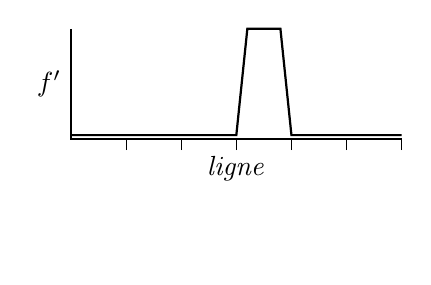
\begin{tikzpicture}[scale=1.4,baseline=-1.5cm]
\draw (0,1) -- node[left] {$f'$} (0,0) -- node[below,yshift=-1mm] {\textit{ligne}} (3,0);
\draw[thick] (0,1pt) -- (1.5,1pt) -- (1.6,1) -- (1.9,1) -- (2,1pt) -- (3,1pt);
\foreach \x in {.5,1,1.5,2,2.5,3}
  \draw[thin] (\x,-1mm) -- (\x,0);
\end{tikzpicture}
\caption{Dérivée première de l'intensité de l'image}
%\caption{First derivative of edge intensity}
\label{fig.edge-first}
\end{minipage}
\hspace{\fill}
\begin{minipage}{.5\textwidth}
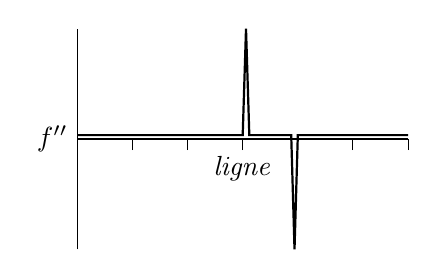
\begin{tikzpicture}[scale=1.4]
\draw (0,-1) -- node[left] {$f''$} (0,1);
\draw (0,0) -- node[below,yshift=-1mm] {\textit{ligne}} (3,0);
\draw[thick] (0,1pt) -- (1.5,1pt) -- (1.53,1) -- (1.56,1pt) -- (1.94,1pt) -- (1.97,-1) -- (2,1pt) -- (3,1pt);
\foreach \x in {.5,1,1.5,2,2.5,3}
  \draw[thin] (\x,-1mm) -- (\x,0);
\end{tikzpicture}
\caption{Dérivée seconde de l'intensité de l'image}
\label{fig.edge-second}
\end{minipage}
\end{figure}

Étant donné que le calcul de la moyenne est un opérateur d'intégration qui \emph{gomme} les changements brusques d'intensité, il n'est pas surprenant que l'opérateur différentiel puisse être utilisé pour \emph{détecter} les changements brusques qui représentent les bords. La figure \ref{fig.edge-intensity} représente l'intensité en fonction du numéro de ligne pour une colonne de la figure \ref{fig.edge}, bien que les intensités soient représentées sous forme de lignes et non par un nuage de points. L'intensité ne varie pas pour les trois premiers pixels, puis elle croit rapidement et enfin reste constante et maximale. La dérivée première $f'$ d'une fonction $f$ est nulle lorsque $f$ est constante, positive lorsque $f$ est croissante et négative lorsque $f$ est décroissante. C'est ce que montre la figure \ref{fig.edge-first}. On peut détecter un bord en recherchant une augmentation ou une diminution rapide de la dérivée première de l'intensité de l'image.

Dans la pratique, il est préférable d'utiliser la dérivée seconde. La figure ~\ref{fig.edge-second} montre un tracé de $f''$, la dérivée de $f'$ dans la figure ~\ref{fig.edge-first}. Le pic positif suivi du pic négatif indique une transition du foncé vers le clair ; si la transition se faisait du clair vers le foncé, le pic négatif précéderait le pic positif.

Il existe de nombreux opérateurs de dérivation discrets. L'un d'entre eux est le \emph{filtre de Sobel}\index{traitement d'image!filtre de Sobel}. Il est simple et efficace et se décline en deux filtres, l'un pour détecter les bords horizontaux (à gauche) et l'autre pour détecter les bords verticaux (à droite) :
\[
\begin{array}{c@{\hspace{4em}}c}
\left[
\begin{array}{rrr}
-1 & -2 & -1\\
0 & 0 & 0\\
1 & 2 & 1\\
\end{array}
\right]
&
\left[
\begin{array}{rrr}
-1 & 0 & 1\\
-2 & 0 & 2\\
-1 & 0 & 1\\
\end{array}
\right]\,.
\end{array}
\]
Une caractéristique d'un filtre de dérivation est que la somme de ses éléments doit être égale à zéro. En effet, si l'opérateur est appliqué à un pixel dont l'intensité est la même que celle de tous ses voisins, le résultat doit être nul. Regardez à nouveau les figures \ref{fig.edge-intensity} et \ref{fig.edge-first} où la dérivée est nulle lorsque l'intensité est constante.

Lorsque les filtres de Sobel sont appliqués au tableau de pixels de la figure \ref{fig.edge}, le résultat obtenu montre que l'on détecte clairement la présence d'un bord horizontal (figure \ref{fig.sobel-horizontal}) mais pas de bord vertical (figure \ref{fig.sobel-vertical}).

\begin{figure}
\begin{minipage}{.45\textwidth}
\begin{tabular}{r@{\hspace{4pt}}r@{\hspace{6pt}}r@{\hspace{6pt}}r@{\hspace{6pt}}r@{\hspace{6pt}}r@{\hspace{6pt}}r@{\hspace{6pt}}r@{\hspace{6pt}}r@{\hspace{6pt}}r@{\hspace{6pt}}r}
& $\scriptstyle 0$ & $\scriptstyle 1$ & $\scriptstyle 2$ & $\scriptstyle 3$ & $\scriptstyle 4$ & $\scriptstyle 5$\\
$\scriptstyle 0$ &    $0$ &   $0$ &   $0$ &   $0$ &   $0$ &   $0$ \\
$\scriptstyle 1$ &    $0$ &   $0$ &   $0$ &   $0$ &   $0$ &   $0$ \\
$\scriptstyle 2$ &    $0$ &  $80$ &  $80$ &  $80$ &  $80$ &   $0$ \\
$\scriptstyle 3$ &    $0$ &  $80$ &  $80$ &  $80$ &  $80$ &   $0$ \\
$\scriptstyle 4$ &    $0$ &   $0$ &   $0$ &   $0$ &   $0$ &   $0$ \\
$\scriptstyle 5$ &    $0$ &   $0$ &   $0$ &   $0$ &   $0$ &   $0$ \\
\end{tabular}
\caption{Résultat de l’application du filtre de  Sobel pour les bords horizontaux}\label{fig.sobel-horizontal}
\end{minipage}
\hspace{\fill}
\begin{minipage}{.45\textwidth}
\begin{tabular}{r@{\hspace{4pt}}r@{\hspace{6pt}}r@{\hspace{6pt}}r@{\hspace{6pt}}r@{\hspace{6pt}}r@{\hspace{6pt}}r@{\hspace{6pt}}r@{\hspace{6pt}}r@{\hspace{6pt}}r@{\hspace{6pt}}r}
& $\scriptstyle 0$ & $\scriptstyle 1$ & $\scriptstyle 2$ & $\scriptstyle 3$ & $\scriptstyle 4$ & $\scriptstyle 5$\\
$\scriptstyle 0$ &    $0$ &   $0$ &   $0$ &   $0$ &   $0$ &   $0$ \\
$\scriptstyle 1$ &    $0$ &   $0$ &   $0$ &   $0$ &   $0$ &   $0$ \\
$\scriptstyle 2$ &    $0$ &   $0$ &   $0$ &   $0$ &   $0$ &   $0$ \\
$\scriptstyle 3$ &    $0$ &   $0$ &   $0$ &   $0$ &   $0$ &   $0$ \\
$\scriptstyle 4$ &    $0$ &   $0$ &   $0$ &   $0$ &   $0$ &   $0$ \\
$\scriptstyle 5$ &    $0$ &   $0$ &   $0$ &   $0$ &   $0$ &   $0$ \\
\end{tabular}
\caption{Résultat de l’application du filtre de Sobel pour les bords verticaux}\label{fig.sobel-vertical}
\end{minipage}
\end{figure}

Les filtres de Sobel sont très puissants car ils peuvent non seulement détecter un bord mais aussi calculer l'angle du bord dans l'image. La figure~\ref{fig.diagonal-edge} montre une image avec un bord oblique allant du coin supérieur gauche au coin inférieur droit de l'image. Les résultats de l'application des deux filtres de Sobel sont présentés dans les figures~\ref{fig.sobel-diagonal-horizontal}--\ref{fig.sobel-diagonal-vertical}. À partir des amplitudes et des signes des éléments de ces tableaux, l'angle du bord peut être calculé comme décrit dans \cite[Sect.~4.3.1]{siegwart}.

\begin{figure}
\begin{tabular}{r@{\hspace{4pt}}r@{\hspace{6pt}}r@{\hspace{6pt}}r@{\hspace{6pt}}r@{\hspace{6pt}}r@{\hspace{6pt}}r@{\hspace{6pt}}r@{\hspace{6pt}}r@{\hspace{6pt}}r@{\hspace{6pt}}r}
& $\scriptstyle 0$ & $\scriptstyle 1$ & $\scriptstyle 2$ & $\scriptstyle 3$ & $\scriptstyle 4$ & $\scriptstyle 5$\\
$\scriptstyle 0$ &    $30$ &   $30$ &   $30$ &   $30$ &   $30$ & $30$ \\
$\scriptstyle 1$ &    \boldmath $50$ &   $30$ &   $30$ &   $30$ &   $30$ & $30$ \\
$\scriptstyle 2$ &    \boldmath $50$ &   \boldmath 50$$ &   $30$ &   $30$ &   $30$ & $30$ \\
$\scriptstyle 3$ &    \boldmath $50$ &   \boldmath $50$ &   \boldmath $50$ &   $30$ &   $30$ & $30$ \\
$\scriptstyle 4$ &    \boldmath $50$ &   \boldmath $50$ &   \boldmath $50$ &   \boldmath $50$ &   $30$ & $30$ \\
$\scriptstyle 5$ &    \boldmath $50$ &   \boldmath $50$ &   \boldmath $50$ &   \boldmath $50$ &   \boldmath $50$ & $30$ \\
\end{tabular}
\caption{Bord oblique}\label{fig.diagonal-edge}
\end{figure}

\begin{figure}
\begin{minipage}{.45\textwidth}
\begin{tabular}{r@{\hspace{4pt}}r@{\hspace{6pt}}r@{\hspace{6pt}}r@{\hspace{6pt}}r@{\hspace{6pt}}r@{\hspace{6pt}}r@{\hspace{6pt}}r@{\hspace{6pt}}r@{\hspace{6pt}}r@{\hspace{6pt}}r}
& $\scriptstyle 0$ & $\scriptstyle 1$ & $\scriptstyle 2$ & $\scriptstyle 3$ & $\scriptstyle 4$ & $\scriptstyle 5$\\
$\scriptstyle 0$ &    $0$ &   $0$ &   $0$ &   $0$ &   $0$ &   $0$ \\
$\scriptstyle 1$ &    $0$ &   \boldmath $60$ &   $20$ &   $0$ &   $0$ &   $0$ \\
$\scriptstyle 2$ &    $0$ &   \boldmath $60$ &   \boldmath $60$ &   $20$ &   $0$ &   $0$ \\
$\scriptstyle 3$ &    $0$ &   $20$ &   \boldmath $60$ &   \boldmath $60$ &   $20$ &   $0$ \\
$\scriptstyle 4$ &    $0$ &   $0$ &   $20$ &   \boldmath $60$ &   \boldmath $60$ &   $0$ \\
$\scriptstyle 5$ &    $0$ &   $0$ &   $0$ &   $0$ &   $0$ &   $0$ \\
\end{tabular}
\caption{Filtre horizontal de Sobel sur un bord oblique}
\label{fig.sobel-diagonal-horizontal}
\end{minipage}
\hspace{\fill}
\begin{minipage}{.45\textwidth}
\begin{tabular}{r@{\hspace{4pt}}r@{\hspace{6pt}}r@{\hspace{6pt}}r@{\hspace{6pt}}r@{\hspace{6pt}}r@{\hspace{6pt}}r@{\hspace{6pt}}r@{\hspace{6pt}}r@{\hspace{6pt}}r@{\hspace{6pt}}r}
& $\scriptstyle 0$ & $\scriptstyle 1$ & $\scriptstyle 2$ & $\scriptstyle 3$ & $\scriptstyle 4$ & $\scriptstyle 5$\\
$\scriptstyle 0$ &    $0$ &   $0$ &   $0$ &   $0$ &   $0$ &   $0$ \\
$\scriptstyle 1$ &    $0$ &   \boldmath $-60$ &   $-20$ &   $0$ &   $0$ &   $0$ \\
$\scriptstyle 2$ &    $0$ &   \boldmath $-60$ &   \boldmath $-60$ &   $-20$ &   $0$ &   $0$ \\
$\scriptstyle 3$ &    $0$ &   $-20$ &   \boldmath $-60$ &   \boldmath $-60$ &   $-20$ &   $0$ \\
$\scriptstyle 4$ &    $0$ &   $0$ &   $-20$ &   \boldmath $-60$ &   \boldmath $-60$ &   $0$ \\
$\scriptstyle 5$ &    $0$ &   $0$ &   $0$ &   $0$ &   $0$ &   $0$ \\
\end{tabular}
\caption{Filtre vertical de Sobel sur un bord oblique}
\label{fig.sobel-diagonal-vertical}
%\caption{Sobel horizontal filter on a diagonal edge}\label{fig.sobel-diagonal-horizontal}
%\caption{Sobel vertical filter on a diagonal edge}\label{fig.sobel-diagonal-vertical}
\end{minipage}
\end{figure}

\begin{framed}
\act{Détection d'un bord}{edge-detection}
\begin{itemize}
\item Imprimez un motif avec un bord saillant (Fig.~\ref{fig.edge-activity}).
\item Adaptez le programme de l'Activity~\ref{act.smoothing} pour que le robot échantillonne et stocke les données du capteur de sol lorsque le robot se déplace sur le motif de gauche à droite. Appliquez un filtre de dérivation aux données collectées.
\item Lors d'un second passage sur le motif, lorsque la valeur de la dérivée n'est pas proche de zéro, le robot devra l'indiquer.
\item Que se passe-t-il si le robot se déplace sur le motif de droite à gauche ?
\item Lors de l'application du filtre, les résultats doivent être stockés dans un tableau séparé, et non dans le tableau utilisé pour stocker les pixels. Pourquoi ?
\end{itemize}
\end{framed}

\begin{figure}
\begin{tikzpicture}
\pic at (-1.9,1.5) { robot };
\draw[fill,gray] (-1,1.3) rectangle +(8pt,12pt);
\draw[->] (2.5, -.4) -- (2.5, -.1);
\draw[fill,color=gray]  (-.5,0) rectangle +(3,3);
\draw[fill,color=black] (2.5,0) rectangle +(3,3);
\end{tikzpicture}
\caption{Activité de détection des bords}\label{fig.edge-activity}
\end{figure}

\section{Détection des coins}\label{s.corners}
\index{traitement d'images!détection des coins}

Le rectangle noir sur fond gris de la Fig.~\ref{fig.corner-image} est plus qu'un simple ensemble de bords ou d'arêtes. Les arêtes verticales forment deux coins avec l'arête horizontale. Nous décrivons ici deux algorithmes permettant d'identifier les coins dans une image. Pour simplifier, nous cherchons à détecter les coins d’un rectangle dont les bords sont parallèles aux bords de l’image.

\begin{figure}
\begin{minipage}{.5\textwidth}

\begin{tikzpicture}[baseline=-1.1cm]
\draw[fill,color=gray]  (0,0) rectangle +(5,2);
\draw[fill,color=black] (1.5,0) rectangle +(2.5,1.5);
\end{tikzpicture}
\caption{Image d'un coin}\label{fig.corner-image}
\end{minipage}
\hspace{\fill}
\begin{minipage}{.5\textwidth}
\begin{tabular}{r@{\hspace{4pt}}r@{\hspace{4pt}}r@{\hspace{4pt}}r@{\hspace{4pt}}r@{\hspace{4pt}}r@{\hspace{4pt}}r@{\hspace{4pt}}r@{\hspace{4pt}}r@{\hspace{4pt}}r@{\hspace{4pt}}r}
& $\scriptstyle 0$ & $\scriptstyle 1$ & $\scriptstyle 2$ & $\scriptstyle 3$ & $\scriptstyle 4$ & $\scriptstyle 5$ & $\scriptstyle 6$ & $\scriptstyle 7$ & $\scriptstyle 8$ & $\scriptstyle 9$ \\
$\scriptstyle 0$ & $30$ & $30$ & $30$ & $30$ & $30$ & $30$ & $30$ & $30$ & $30$ & $30$\\
$\scriptstyle 1$ & $30$ & $30$ & $30$ & $30$ & $30$ & $30$ & $30$ & $30$ & $30$ & $30$\\
$\scriptstyle 2$ & $30$ & $30$ & $30$ & \boldmath $50$ & \boldmath $50$ & \boldmath $50$ & \boldmath $50$ & \boldmath $50$ & $30$ & $30$\\
$\scriptstyle 3$ & $30$ & $30$ & $30$ & \boldmath $50$ & \boldmath $50$ & \boldmath $50$ & \boldmath $50$ & \boldmath $50$ & $30$ & $30$\\
$\scriptstyle 4$ & $30$ & $30$ & $30$ & \boldmath $50$ & \boldmath $50$ & \boldmath $50$ & \boldmath $50$ & \boldmath $50$ & $30$ & $30$\\
$\scriptstyle 5$ & $30$ & $30$ & $30$ & \boldmath $50$ & \boldmath $50$ & \boldmath $50$ & \boldmath $50$ & \boldmath $50$ & $30$ & $30$\\
\end{tabular}
\caption{Réseau de pixels d'un coin}\label{fig.corner-pixels}
\end{minipage}
\end{figure}

Nous savons comment détecter des bords dans une image. Un coin est défini par l'intersection d'un bord vertical et d'un bord horizontal. Figure~\ref{fig.corner-pixels} est le tableau de $6\times 10$ pixels pour l'image de la Fig.~\ref{fig.corner-image}. Si nous appliquons les filtres de détection des bords de Sobel à ce tableau de pixels, nous obtenons deux bords verticaux  (Fig.~\ref{fig.corner-vertical}) et un bord horizontal (Fig.~\ref{fig.corner-horizontal}).

Pour déterminer les intersections, on prend la moyenne des valeurs absolues des deux tableaux obtenus en appliquant les filtres de détection de bords de Sobel. Les pixels dont la moyenne des valeurs absolues dépasse un seuil sont nos intersections. Avec un seuil de $60$, les arêtes se croisent aux pixels $(2,3)$ et $(2,7)$ qui sont nos coins.

\begin{figure}
\begin{minipage}{.5\textwidth}
\begin{tabular}{r@{\hspace{4pt}}r@{\hspace{4pt}}r@{\hspace{4pt}}r@{\hspace{4pt}}r@{\hspace{4pt}}r@{\hspace{4pt}}r@{\hspace{4pt}}r@{\hspace{4pt}}r@{\hspace{4pt}}r@{\hspace{4pt}}r}
& $\scriptstyle 0$ & $\scriptstyle 1$ & $\scriptstyle 2$ & $\scriptstyle 3$ & $\scriptstyle 4$ & $\scriptstyle 5$ & $\scriptstyle 6$ & $\scriptstyle 7$ & $\scriptstyle 8$ & $\scriptstyle 9$ \\
$\scriptstyle 0$ & $0$ & $0$ & $0$ & $0$ & $0$ & $0$ & $0$ & $0$ & $0$ & $0$\\
$\scriptstyle 1$ & $0$ & $0$ & \boldmath $20$ & \boldmath $20$ & $0$ & $0$ & $0$ & \boldmath $-20$ & \boldmath $-20$ & $0$\\
$\scriptstyle 2$ & $0$ & $0$ & \boldmath $60$ & \boldmath $60$ & $0$ & $0$ & $0$ & \boldmath $-60$ & \boldmath $-60$ & $0$\\
$\scriptstyle 3$ & $0$ & $0$ & \boldmath $80$ & \boldmath $80$ & $0$ & $0$  & $0$ & \boldmath $-80$ & \boldmath $-80$ & $0$\\
$\scriptstyle 4$ & $0$ & $0$ & \boldmath $80$ & \boldmath $80$ & $0$ & $0$  & $0$ & \boldmath $-80$ & \boldmath $-80$ & $0$ \\
$\scriptstyle 5$ & $0$ & $0$ & $0$ & $0$ & $0$ & $0$ & $0$ & $0$ & $0$ & $0$\\
\end{tabular}
\caption{Bords verticaux}\label{fig.corner-vertical}
\end{minipage}
\hspace{\fill}
\begin{minipage}{.5\textwidth}
\begin{tabular}{r@{\hspace{4pt}}r@{\hspace{4pt}}r@{\hspace{4pt}}r@{\hspace{4pt}}r@{\hspace{4pt}}r@{\hspace{4pt}}r@{\hspace{4pt}}r@{\hspace{4pt}}r@{\hspace{4pt}}r@{\hspace{4pt}}r}
& $\scriptstyle 0$ & $\scriptstyle 1$ & $\scriptstyle 2$ & $\scriptstyle 3$ & $\scriptstyle 4$ & $\scriptstyle 5$ & $\scriptstyle 6$ & $\scriptstyle 7$ & $\scriptstyle 8$ & $\scriptstyle 9$ \\
$\scriptstyle 0$ & $0$ & $0$ & $0$ & $0$ & $0$ & $0$ & $0$ & $0$ & $0$ & $0$\\
$\scriptstyle 1$ & $0$ & $0$ & \boldmath $20$ & \boldmath $60$ & \boldmath $80$ & \boldmath $80$ & \boldmath $80$ & \boldmath $60$ & \boldmath $20$ & $0$\\
$\scriptstyle 2$ & $0$ & $0$ & \boldmath $20$ & \boldmath $60$ & \boldmath $80$ & \boldmath $80$ & \boldmath $80$ & \boldmath $60$ & \boldmath $20$ & $0$\\
$\scriptstyle 3$ & $0$ & $0$ & $0$ & $0$ & $0$ & $0$ & $0$ & $0$ & $0$ & $0$\\
$\scriptstyle 4$ & $0$ & $0$ & $0$ & $0$ & $0$ & $0$ & $0$ & $0$ & $0$ & $0$\\
$\scriptstyle 5$ & $0$ & $0$ & $0$ & $0$ & $0$ & $0$ & $0$ & $0$ & $0$ & $0$\\
\end{tabular}
\caption{Bord horizontal}\label{fig.corner-horizontal}
\end{minipage}
\end{figure}

Une zone uniforme, un bord et un coin peuvent être distingués en analysant les voisins d'un pixel. Pour les pixels d'une zone uniforme, tous les voisins du pixel ont approximativement la même intensité. Pour les pixels d'un bord, les intensités des voisins du pixel sont très différentes dans une direction et similaires dans l'autre. Pour les pixels qui soont des coins, les intensités des voisins du pixel présentent peu de similitudes. . Les pixels qui n’ont pas 8 voisins ne sont pas considérés ici. Pour  une zone, un bord ou un coin, le nombre minimal de pixels voisins similaires ne peut pas être nul. Pour détecter un coin, on  peut donc compter le nombre de voisins similaires pour chaque pixel à l'intérieur de l'image, c'est-à-dire ceux qui ont 8 voisins, trouver le nombre minimal non nul de voisins similaires de l'image et identifier comme coins les pixels ayant ce nombre minimal de voisins similaires. La figure \ref{fig.similar-neighbors} montre les décomptes de voisins similaires pour les pixels de la figure \ref{fig.corner-pixels}. Comme prévu, les pixels $(2,3)$ et $(2,7)$ ont le nombre minimum de voisins similaires et ce sont nos pixels de coin.

\begin{figure}
\begin{center}
\begin{tabular}{r@{\hspace{4pt}}r@{\hspace{4pt}}r@{\hspace{4pt}}r@{\hspace{4pt}}r@{\hspace{4pt}}r@{\hspace{4pt}}r@{\hspace{4pt}}r@{\hspace{4pt}}r@{\hspace{4pt}}r@{\hspace{4pt}}r}
& $\scriptstyle 0$ & $\scriptstyle 1$ & $\scriptstyle 2$ & $\scriptstyle 3$ & $\scriptstyle 4$ & $\scriptstyle 5$ & $\scriptstyle 6$ & $\scriptstyle 7$ & $\scriptstyle 8$ & $\scriptstyle 9$ \\
$\scriptstyle 0$ & $0$ & $0$ & $0$ & $0$ & $0$ & $0$ & $0$ & $0$ & $0$ & $0$\\
$\scriptstyle 1$ & $0$ & $8$ & $7$ & $6$ & $5$ & $5$ & $5$ & $6$ & $7$ & $0$\\
$\scriptstyle 2$ & $0$ & $8$ & $6$ & \boldmath $3$ & $5$ & $5$ & $5$ & \boldmath $3$ & $6$ & $0$\\
$\scriptstyle 3$ & $0$ & $8$ & $5$ & $5$ & $8$ & $8$ & $8$ & $5$ & $5$ & $0$\\
$\scriptstyle 4$ & $0$ & $8$ & $5$ & $5$ & $8$ & $8$ & $8$ & $5$ & $5$ & $0$\\
$\scriptstyle 5$ & $0$ & $0$ & $0$ & $0$ & $0$ & $0$ & $0$ & $0$ & $0$ & $0$\\
\end{tabular}
\caption{Nombre de voisins similaires}\label{fig.similar-neighbors}
\end{center}
\end{figure}

\begin{framed}
\act{Détecter un coin}{detect-corner}
\begin{itemize}
\item Mettez en œuvre la détection d'un coin par intersection de bords à l'aide d'un robot équipé de deux capteurs de proximité au sol. Le robot se déplace du bas de l'image de la Fig.~\ref{fig.corner-image} vers le haut. S'il est placé au-dessus du rectangle noir, il ne détecte pas de coin, alors que s'il est placé de manière à ce qu'un capteur soit au-dessus du rectangle noir et l'autre au-dessus du fond gris, il détecte le coin.
\item Mettez en œuvre la détection des coins par la recherche des voisins similaires. Utilisez continuellement l’échantillon courant et l’échantillon précédemment prélevé par les capteurs au sol droit et gauche. Si un seul des quatre échantillons est noir, un coin est détecté.
\end{itemize}
\end{framed}

\section{Reconnaissance des blobs}\label{s.blob}

La figure \ref{fig.blob} montre un \emph{blob} : une zone à peu près circulaire de $12$ pixels de forte intensité sur un fond de faible intensité. Le blob n'a pas de frontière bien définie comme un rectangle. L'avant-dernière ligne montre également deux artefacts de forte intensité qui ne font pas partie du blob, bien qu'ils puissent eux-mêmes représenter des blobs distincts.La figure \ref{fig.blob-with-noise} montre les pixels après l'ajout d'un bruit aléatoire. Notre objectif est d'identifier le blob en présence de bruit, sans dépendre d'un seuil d'intensité prédéfini et en ignorant les artefacts.  Le robot doit pouvoir accomplir sa tâche quelles que soient les conditions d'éclairage de l'environnement. Il est donc important que la tâche d'identification soit indépendante de l'intensité globale.

\begin{figure}
\begin{minipage}{.5\textwidth}
\begin{tabular}{r@{\hspace{4pt}}r@{\hspace{4pt}}r@{\hspace{4pt}}r@{\hspace{4pt}}r@{\hspace{4pt}}r@{\hspace{4pt}}r@{\hspace{4pt}}r@{\hspace{4pt}}r@{\hspace{4pt}}r@{\hspace{4pt}}r}
& $\scriptstyle 0$ & $\scriptstyle 1$ & $\scriptstyle 2$ & $\scriptstyle 3$ & $\scriptstyle 4$ & $\scriptstyle 5$ & $\scriptstyle 6$ & $\scriptstyle 7$ & $\scriptstyle 8$ & $\scriptstyle 9$ \\
$\scriptstyle 0$ & $30$ & $30$ & $30$ & $30$ & $30$ & $30$ & $30$ & $30$ & $30$ & $30$\\
$\scriptstyle 1$ & $30$ & $30$ & $30$ & $30$ & \boldmath $80$ & \boldmath $80$ & $30$ & $30$ & $30$ & $30$\\
$\scriptstyle 2$ & $30$ & $30$ & $30$ & \boldmath $80$ & \boldmath $80$ & \boldmath $80$ & \boldmath $80$ & $30$ & $30$ & $30$\\
$\scriptstyle 3$ & $30$ & $30$ & $30$ & \boldmath $80$ & \boldmath $80$ & \boldmath $80$ & \boldmath $80$ & $30$ & $30$ & $30$\\
$\scriptstyle 4$ & \boldmath $80$ & $30$ & $30$ & $30$ & \boldmath $80$ & \boldmath $80$ & $30$ & $30$ & $30$ & \boldmath $80$\\
$\scriptstyle 5$ & $30$ & $30$ & $30$ & $30$ & $30$ & $30$ & $30$ & $30$ & $30$ & $30$\\
\end{tabular}
\caption{Blob}\label{fig.blob}
\end{minipage}
\hspace{\fill}
\begin{minipage}{.5\textwidth}
\begin{tabular}{r@{\hspace{4pt}}r@{\hspace{4pt}}r@{\hspace{4pt}}r@{\hspace{4pt}}r@{\hspace{4pt}}r@{\hspace{4pt}}r@{\hspace{4pt}}r@{\hspace{4pt}}r@{\hspace{4pt}}r@{\hspace{4pt}}r}
& $\scriptstyle 0$ & $\scriptstyle 1$ & $\scriptstyle 2$ & $\scriptstyle 3$ & $\scriptstyle 4$ & $\scriptstyle 5$ & $\scriptstyle 6$ & $\scriptstyle 7$ & $\scriptstyle 8$ & $\scriptstyle 9$ \\
$\scriptstyle 0$ & $46$ & $42$ & $40$ & $50$ & $46$ & $44$ & $40$ & $33$ & $30$ & $34$\\
$\scriptstyle 1$ & $32$ & $46$ & $46$ & $46$ & \boldmath $67$ & \boldmath $73$ & $39$ & $47$ & $39$ & $30$\\
$\scriptstyle 2$ & $33$ & $40$ & $40$ & \boldmath $73$ & \boldmath $68$ & \boldmath $63$ & \boldmath $73$ & $44$ & $42$ & $31$\\
$\scriptstyle 3$ & $35$ & $41$ & $50$ & \boldmath $67$ & \boldmath $60$ & \boldmath $71$ & \boldmath $60$ & $37$ & $30$ & $49$\\
$\scriptstyle 4$ & \boldmath $68$ & $46$ & $32$ & $44$ & \boldmath $61$ & \boldmath $77$ & $48$ & $42$ & $45$ & \boldmath $62$\\
$\scriptstyle 5$ & $39$ & $37$ & $38$ & $34$ & $33$ & $40$ & $35$ & $37$ & $34$ & $32$\\
\end{tabular}
\caption{Blob avec bruit}\label{fig.blob-with-noise}
\end{minipage}
\end{figure}

Pour ignorer le bruit sans avoir prédéfini de seuil, nous utilisons l'intensité moyenne de l'imagee pour choisir un seuil. Pour séparer les blobs les uns des autres, nous trouvons d'abord un pixel dont l'intensité est supérieure au seuil, puis nous agrandissons le blob en ajoutant les pixels voisins dont l'intensité est supérieure au seuil. Pour l'image bruitée de la Fig.~\ref{fig.blob-with-noise}, l'intensité moyenne est de $54$. Étant donné que le blob occupe vraisemblablement une partie relativement petite de l'arrière-plan, il peut être judicieux de choisir un seuil légèrement supérieur à la moyenne, par exemple $60$.

La figure \ref{fig.blob-after-threshold} montre l'image après avoir attribué $0$ à tous les pixels en dessous du seuil. Le blob a été détecté, mais les deux artefacts aussi. L'algorithme~\ref{alg.blob} permet d'isoler un seul blob. Tout d'abord, recherchez un pixel qui n'est pas nul ; en commençant en haut à gauche, on obtient ici $p_1=(1,4)$ avec une intensité de $67$. Développez maintenant le blob en ajoutant tous les voisins de $p_1$ dont les intensités sont non nulles ; il s'agit de $p_2=(1,5), p_3=(2,3), p_4=(2,4), p_5=(2,5)$. Continuez à ajouter les voisins non nuls de chaque $p_i$ au blob jusqu'à ce qu'il n'y ait plus de pixels ajoutés. Le résultat sera le blob de $12$ pixels sans les artefacts en $(4,0)$ et $(4,9)$.

L'algorithme a fonctionné parce que le premier pixel non nul trouvé appartenait au blob. S'il y avait eu un pixel isolé non nul en $(1,1)$, cet artefact aurait été détecté comme un blob. Si on disposait d'une estimation de la taille minimale d'un blob, il faudrait vérifier que le blod est au moin de cette taille à la fin de l'algorithme.

\begin{figure}
\begin{minipage}{.5\textwidth}
\begin{tabular}{r@{\hspace{4pt}}r@{\hspace{6pt}}r@{\hspace{6pt}}r@{\hspace{6pt}}r@{\hspace{6pt}}r@{\hspace{6pt}}r@{\hspace{6pt}}r@{\hspace{6pt}}r@{\hspace{6pt}}r@{\hspace{6pt}}r}
& $\scriptstyle 0$ & $\scriptstyle 1$ & $\scriptstyle 2$ & $\scriptstyle 3$ & $\scriptstyle 4$ & $\scriptstyle 5$ & $\scriptstyle 6$ & $\scriptstyle 7$ & $\scriptstyle 8$ & $\scriptstyle 9$ \\
$\scriptstyle 0$ & $ 0$ & $ 0$ & $ 0$ & $ 0$ & $ 0$ & $ 0$ & $ 0$ & $ 0$ & $ 0$ & $ 0$\\
$\scriptstyle 1$ & $ 0$ & $ 0$ & $ 0$ & $ 0$ & $67$ & $73$ & $ 0$ & $ 0$ & $ 0$ & $ 0$\\
$\scriptstyle 2$ & $ 0$ & $ 0$ & $ 0$ & $73$ & $68$ & $63$ & $73$ & $ 0$ & $ 0$ & $ 0$\\
$\scriptstyle 3$ & $ 0$ & $ 0$ & $ 0$ & $67$ & $60$ & $71$ & $60$ & $ 0$ & $ 0$ & $ 0$\\
$\scriptstyle 4$ & $68$ & $ 0$ & $ 0$ & $ 0$ & $61$ & $77$ & $ 0$ & $ 0$ & $ 0$ & $62$\\
$\scriptstyle 5$ & $ 0$ & $ 0$ & $ 0$ & $ 0$ & $ 0$ & $ 0$ & $ 0$ & $ 0$ & $ 0$ & $ 0$\\
\end{tabular}
\caption{Blob après le seuil}\label{fig.blob-after-threshold}
\end{minipage}
\hspace{\fill}
\begin{minipage}{.5\textwidth}

\begin{tikzpicture}[baseline=-4mm]
\path (0,2) rectangle +(2,.8);
\draw[fill,color=gray]  (0,0) rectangle +(5,2);
\draw[fill,color=black] (1,0) rectangle +(1.5,2);
\draw[fill,color=black] (3.5,0) rectangle +(.5,2);
\end{tikzpicture}
\caption{Blob à détecter}\label{fig.blob-for-activity}
\end{minipage}
\end{figure}

\begin{figure}
\begin{alg}{Détection d'un blob}{blob}           
&\idv{}entier seuil&\\
&\idv{}pixel p&\\
&\idv{}ensemble non-exploré \ass ensemble-vide&\\
&\idv{}ensemble blob \ass ensemble-vide&\\
\hline
\stl{}&fixer le seuil à l'intensité moyenne&\\
\stl{}&mettre les pixels dont l'intensité est inférieurs au seuil à zéro&\\
\stl{}&trouver un pixel non nul et l'jouter à l'ensemble non-exploré&\\
\stl{}&tant que non-exploré n'est pas vide&\\
\stl{}&\idc{}p \ass un élément de non-exploré&\\
\stl{}&\idc{}ajouter p à blob&\\
\stl{}&\idc{}retirer p de non-exploré&\\
\stl{}&\idc{}ajouter les voisins non nuls de p à non-exploré&\\
\end{alg}
\end{figure}

Vérifiez que l'algorithme~\ref{alg.blob} n'est pas sensible au niveau d'intensité en soustrayant la valeur constante $20$ à tous les éléments de l'image bruitée (Fig.~\ref{fig.blob-with-noise}) et en réexécutant l'algorithme. Celui-ci devrait toujours identifier les mêmes pixels comme appartenant au blob.

\begin{framed}
\act{Détection d'un blob}{blob}
\begin{itemize}
\item Ecrivez un programme qui permet au robot d'échantillonner le capteur de sol lorsqu'il se déplace de gauche à droite sur le motif de la Fig.~\ref{fig.blob-for-activity}.
\item Calculez l'intensité moyenne des données relevées et fixer le seuil à la moyenne.
\item Lors d'un deuxième passage sur le motif, après avoir détecté le premier élément du rectangle noir qui est en dessous du seuil, le robot fournit une indication (une lumière ou un son) tant qu'il se déplace sur le rectangle.
\item Le robot devra considérer le second rectangle noir comme un artefact et l'ignorer.
\end{itemize}
\end{framed}

\begin{framed}
\act{Reconnaître une porte}{recognize}
\begin{itemize}
\item Dans la figure~\ref{fig.door}, le rectangle gris représente une porte ouverte dans un mur sombre représenté par les rectangles noirs. La figure~\ref{fig.not-a-door} représente un mur sombre (en noir) entre deux portes ouvertes (en gris). Si vous exécutez le programme à partir de l'activité~\ref{act.edge-detection}, vous verrez que deux bords sont détectées dans les deux cas. Modifiez le programme pour que le robot puisse faire la distinction entre les deux situations.
\end{itemize}
\end{framed}

\begin{figure}
\begin{minipage}{.45\textwidth}

\begin{tikzpicture}
\draw[fill,color=black] (0,0) rectangle +(1.5,2);
\draw[fill,color=gray]  (1.5,0) rectangle +(2,2);
\draw[fill,color=black] (3.5,0) rectangle +(1.5,2);
\end{tikzpicture}
\caption{Reconnaître la porte}\label{fig.door}
\end{minipage}
\hspace{\fill}
\begin{minipage}{.45\textwidth}

\begin{tikzpicture}[baseline=-3mm]
\path (0,2) rectangle +(2,.6);
\draw[fill,color=gray]  (0,0) rectangle +(1.5,2);
\draw[fill,color=black] (1.5,0) rectangle +(2,2);
\draw[fill,color=gray]  (3.5,0) rectangle +(1.5,2);
\end{tikzpicture}
\caption{Il ne s'agit pas d'une porte}\label{fig.not-a-door}
\end{minipage}
\end{figure}

\section{Résumé}

Chez les êtres humains et la plupart des animaux, la vision est le capteur le plus important et une grande partie du cerveau est consacrée à l'interprétation des signaux visuels. Les robots peuvent utiliser la vision pour effectuer des tâches avancées dans un environnement qui change constamment. La technologie des caméras numériques est très avancée et les caméras peuvent transmettre des images à haute résolution sous forme de matrices de pixels aux ordinateurs des robots. Les algorithmes de traitement des images numériques améliorent et interprètent ces images.

Les algorithmes d'amélioration suppriment le bruit, améliorent le contraste et effectuent d'autres opérations qui ne dépendent pas des objets apparaissant dans l'image. Ils utilisent des filtres spatiaux qui modifient l'intensité de chaque pixel en fonction de l'intensité de ses voisins. La modification de l'histogramme utilise la distribution globale des intensités d'image pour modifier les pixels isolement.

Après l'amélioration de l'image, d'autres algorithmes permettent d'identifier les objets dans l'image. Ils servent à détecter des propriétés géométriques simples telles que les bords et les coins, pour ensuite identifier les objets qui apparaissent dans l'image.

\section{Lecture complémentaire}

Gonzalez et Woods \cite{GW} est un manuel complet sur le traitement des images numériques qui reprend les bases mathématiques requises. Russ \cite{russ} est un ouvrage de référence sur le traitement des images. Szeliski \cite{szeliski} est un livre sur la vision par ordinateur qui va au-delà du traitement d'images et se concentre sur la construction de modèles 3D d'images. Pour les applications du traitement d'images en robotique, voir \cite[Chapter~4]{siegwart}.
